\chapter[The advection effect]{The advection effect as a driver of microbial biogeography}
\label{ch:advection}

\previouslypublished{Sections of this chapter have been previously published in}

\section{Summary}

\section{Introduction}

The central goal of microbial biogeography is to understand how the distribution and abundance of microorganisms are shaped by their physical context.
The Baas Becking hypothesis --- that ``\textit{everything is everywhere}, but, \textit{the environment selects} \cite{Becking:1934um, deWit:2006de}'' --- posits that the rapid dispersal of microorganisms means microbial community structure is determined entirely by environmental selection.
This stands in contrast to macroorganism biogeography, which has long been recognised as being under the control of historical (in addition to contemporary environmental) factors, particularly spatial influences such as barriers to dispersal.
Microbial biogeography studies have begun to show that historical factors may also shape the distribution of microorganisms \cite{Martiny:2006jy}, e.g.\ a correlation between spatial and genetic distance (a ``distance effect'') in fluorescent \genus{Pseudomonas} strains in soils \cite{Cho:2000tn}.
This study, among others \cite{Ramette:2007bb,Storch:2008tq}, also demonstrated the importance of taxonomic resolution in describing such biogeographic patterns.
Other studies have found that dispersal potential varies between microbial species, leading to different or absent distance effects \cite{Bissett:2010wj}.
When combined with contemporary environmental selection (``environment effect''), distance effects explain some but not all variation between microbial communities, and the mechanism(s) by which a distance effect arises are not always clear \cite{Hanson:2012cb}.

In the ocean, several recent studies have found that microbial communities can be endemic to hydrographically distinct water masses.
Surveys in the Arctic \cite{Galand:2009hy} and North Atlantic \cite{Agogue:2011fm} oceans have found that bacterial assemblages within the same water mass can be similar across a range of thousands of kilometres, but assemblages can differ between water masses across a range of hundreds of meters.
Water masses are defined by their distinct physicochemical properties, so such patterns do not directly imply the existence of factors beyond environmental selection.
However, in some cases a water mass-community relationship has been shown to persist even when environment effects are statistically controlled for \cite{Hamilton:2008tp, Hamdan:2013ko}.

During the study on the biogeographic effect of the \ac{PF} described earlier in this volume, it was found that microbial communities in surface waters of the Mertz Glacier region, a site of deep water formation, were very similar to those at the bottom of the water column, despite the very different environmental conditions (see \secreft{ch:deepappendix}).
One hypothesis explaining both this observation and water mass endemicity is that microbial assemblages are influenced by the advection (physical transport) of cells by ocean currents. 
Higher dispersal rates cause the microbial community composition at a given site to increasingly resemble the dispersed colonisers, and less reflect local environmental selection and stochastic effects such as genetic drift \cite{Hanson:2012cb}.
Hence, it would be expected that locations that are closely connected by advection (e.g.\ those within the same water mass, or different levels of the water column at a site of deep water formation) would have more similar compositions than those that are not, even when the environment effect is accounted for.
Indeed, advection is often invoked to explain observations of microbial diversity or abundance which do not seem attributable to environmental selection \citep[e.g.][]{Sul:2013in, Ghiglione:2012ei, Giebel:2009hr, Lauro:2007bf}.
The exchange of very small volumes of water between marine microbial mesocosms has been found to greatly reduce their \textbeta-diversity even under consistent environmental conditions \cite{Declerck:2013cz}.
This suggests that advection of even small numbers of cells could have a large homogenizing effect independent of environmental selection.
However, the existence of a relationship between advection and community composition that is independent of environment and distance effects has not been directly tested.

The \ac{SO} is composed of several water masses, which are physicochemically distinct but linked by circulation (see \secreft{ch:intro} for a full description; see also \autoref{fig:advectionsamplemap}).
This study aimed to determine whether advection shapes the community structure of bacteria and archaea, independent of environment and distance effects.
By sampling each of the \ac{SO} water masses (depths from surface to \textapprox{}6 km), dissimilarity between microbial communities over a large spatial distance (\textapprox{}3000 km) and range of environments could be determined, in order to test whether advection played a role in shaping their composition.

\section{Methods}

\subsection{Sampling}

\begin{figure}
  \centering
  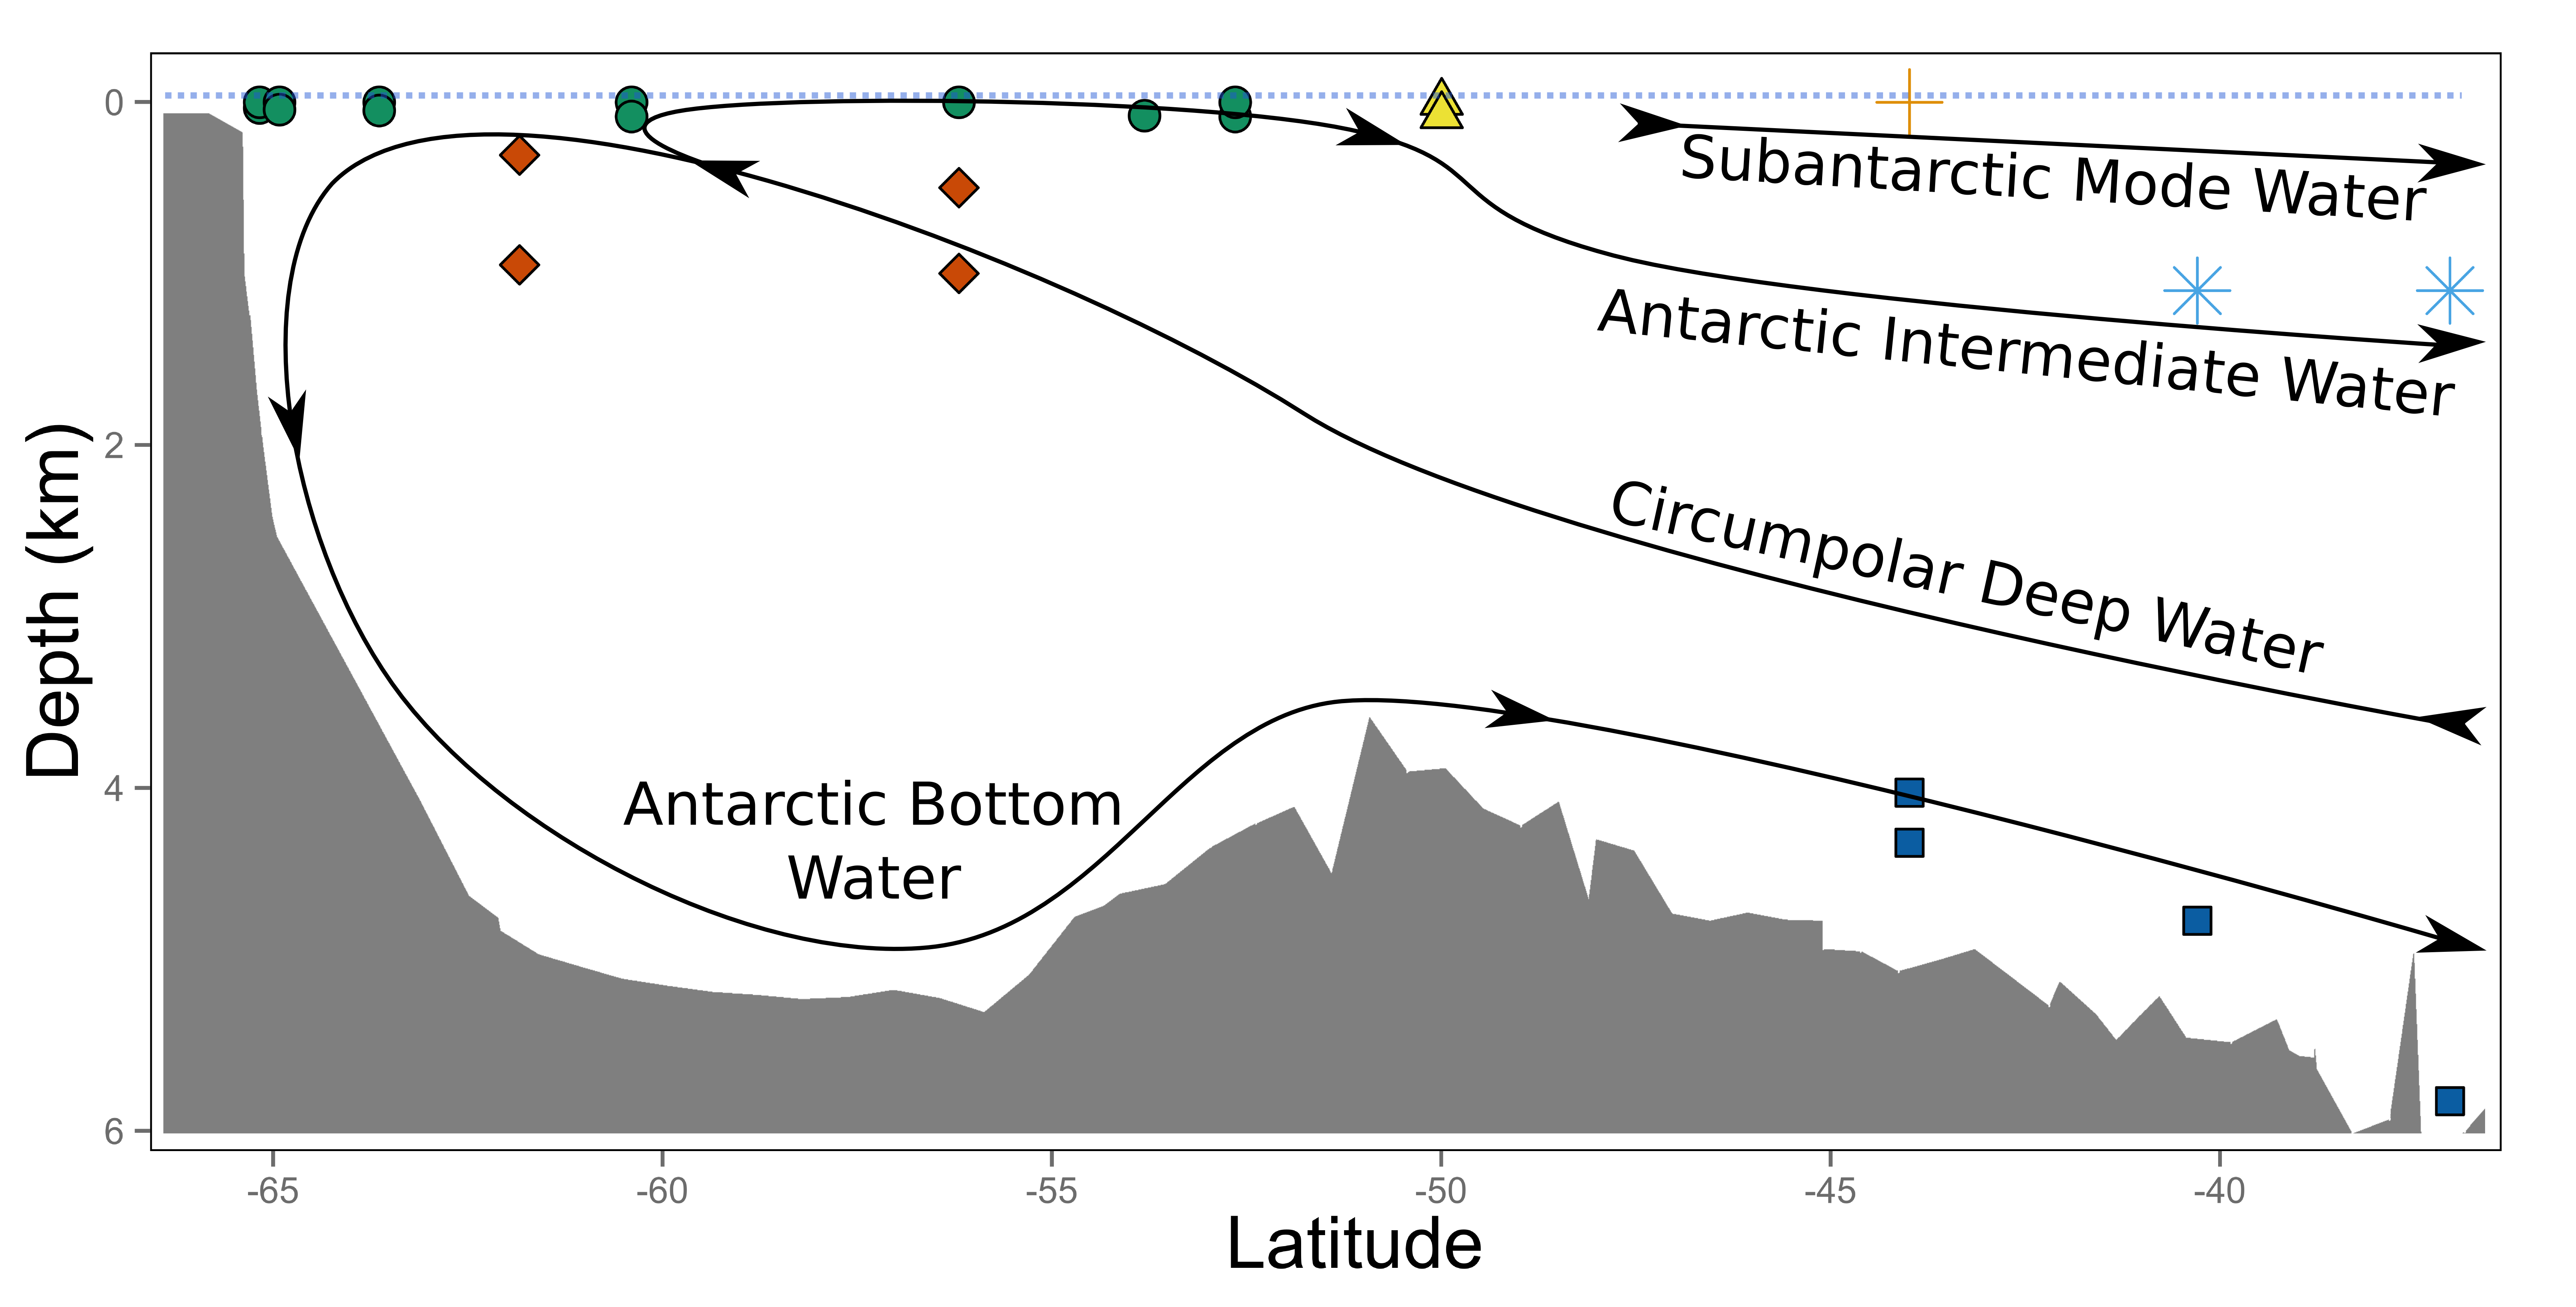
\includegraphics[width=\textwidth]{../advection/advectionsamplemap.png}
  \caption[Map showing sites of samples used in the advection study]{Antarctic Intermediate Waters (AAIW), light blue stars; Subantarctic Mode Water (SAMW), orange crosses; Antarctic Bottom Water (AABW), dark blue squares; Antarctic Zone (AZ), green circles; Polar Frontal Zone (PFZ), yellow triangles; Circumpolar Deep Water (CDW), red diamonds; sea surface, blue dashed horizontal line. Bathymetry is an approximate representation for 115\textdegree{} E, and is indicative only.}
  \label{fig:advectionsamplemap}
\end{figure}

Sampling\footnote{Sampling was performed by David Wilkins, Timothy J.\ Williams and Sheree Yau.} was conducted on board the RSV \textit{Aurora Australis} during cruise V3 from January 20th--February 7th 2012.
This cruise occupied a latitudinal transect from waters north of Cape Poinsett, Antarctica (65\textdegree{} S) to south of Cape Leeuwin, Australia (37\textdegree{} S) within a longitudinal range of 113--115\textdegree{} E.

Sampling was performed as described in \citet{Wilkins:2012wg}, with sites and depths selected to provide coverage of all major \ac{SO} water masses.
At each surface station, \textapprox{}250--560 L of seawater was pumped from \textapprox{}1.5--2.5 m depth.
At some surface stations, an additional sample was taken from the \ac{DCM}, as determined by chlorophyll fluorescence measurements taken from a \ac{CTD} cast at each station.
Samples of mesopelagic and deeper waters (\textapprox{}120--240 L) were also collected at some stations using Niskin bottles attached to the \ac{CTD}.
Sampling depths were selected based on temperature, salinity and dissolved oxygen profiles to capture water from the targeted water masses.
Profiles were generated on the \ac{CTD} descent, and samples collected on the ascent at the selected depths.
Deep water masses were identified by the following criteria: \ac{CDW} = oxygen minimum (\ac{UCD}) or salinity maximum (\ac{LCD}); \ac{AABW} = deep potential temperature minimum; \ac{AAIW} = salinity minimum \cite{Foldvik:1988gp}.
Surface zones were identified relative to the major fronts of the \ac{SO}, which are marked by strong latitudinal gradients in temperature and salinity \cite{Sokolov:2002tc, Orsi:1995va}.
The \ac{AZ} lies south of the \ac{PF} (\textapprox{}51\textdegree{} S at the time of sampling), while the \ac{PFZ} lies between the \ac{PF} and the \ac{SAF}.
\ac{SAMW} overlays \ac{AAIW} north of the \ac{SAF}.
In total, 25 samples from the \ac{AZ}, \ac{PFZ}, \ac{SAMW}, \ac{AAIW}, \ac{CDW} and \ac{AABW} were collected for this study \figref{fig:advectionsamplemap}.

Seawater samples were prefiltered through a 20 \micron{} plankton net, then filtrate was captured on sequential 3.0 \micron{} 0.8 \micron{} and 0.1 \micron{} 293 mm polyethersulfone membrane filters (Pall, Port Washington, USA), and immediately stored at $-20$ $^\circ$C \cite{Rusch:2007ez,Ng:2010cd}.

\subsection{DNA extraction}

DNA extraction was performed using a modified version of the phenol-chloroform method described in \citet{Rusch:2007ez}.
Samples were thawed in a 37 \textdegree{}C water bath.
Half of the storage buffer (\textapprox{}10 mL) was decanted into a clean 50 mL centrifuge tube.
If the volume decanted was less than 10 mL, the difference was made with sterile water (Sigma-Aldrich, St.\ Louis, USA).
An equal volume of 50\% sucrose lysis buffer (50 mM TRIS-HCl, 40 mM EDTA, 0.75 M Sucrose, pH 8) was added such that the final concentration was 25\% sucrose lysis buffer.
A small pinch of lysozyme (Sigma-Aldrich, St.\ Louis, USA) (final concentration \textapprox{}2.5 mg/mL) and 1 mL TRIS-EDTA (10 mM TRIS, 1 mM EDTA, pH 8) was added.

The filter membrane was removed from the storage tube and cut in half aseptically.
One half was returned to the storage tube, which was refrozen at $-80$ \textdegree{}C.
The remaining half was cut in half again, and one quarter-filter placed atop the other such that the biomass (filtrand) on each piece was facing outwards.
Keeping the filters together, they were cut into very fine (\textapprox{}3 mm by 10 mm) strips, which were placed in the 50 mL centrifuge tube containing the buffer and lysozyme mixture.
This tube was mixed by gentle inversion, then tapped such that all filter strips collected at the bottom of the tube and were covered by lysis buffer.
The tube was then incubated in a 37 \textdegree{}C shaking water bath at 275 RPM for 30--60 min.

200 \microlitre{} of 20 mg/mL Proteinase K (Sigma-Aldrich, St.\ Louis, USA) was added to the tube, which was mixed by gentle inversion.
The tube was gently tapped such that all filter strips collected at the bottom covered by lysis buffer.
The tube was then subjected to three freeze-thaw cycles, each cycle consisting of 20--30 min in a $-80$ \textdegree{}C freezer followed by 20--30 min in a 55 \textdegree{}C water bath.
After the final complete thaw, 200 \microlitre{} of 20 mg/mL Proteinase K and 2 mL of 10\% SDS (Sigma-Aldrich, St.\ Louis, USA) were added to the tube.
The tube was mixed by gentle inversion then gently tapped such that all filter strips collected at the bottom covered by lysis buffer.
It was then incubated in a 55 \textdegree{}C shaking water bath at 175 RPM for two hours.

The supernatant was pipetted from the tube using a genomic tip and split evenly into two new 50 mL centrifuge tubes.
An equal volume of buffer-saturated (10 mM TRIS HCl, 1 mM EDTA, pH 8) phenol (Sigma-Aldrich, St.\ Louis, USA) was added to each of the tubes, which were mixed by gentle inversion.
The mixtures were then fractionated in a fixed-angle rotor centrifuge for 15 min at 3700 RPM at room temperature.
The bottom layer of each tube was removed by pipette into a new 50 mL centrifuge tube.
Each of these two tubes was then made to 50 mL with sterile water (Sigma-Aldrich, St.\ Louis, USA).
After mixing by gentle inversion, each 50 mL mixture was then split evenly into two new 50 mL centrifuge tubes, resulting in four tubes each containing 25 mL of mixture.
These tubes were then made to 50 mL with 1-propanol (Sigma-Aldrich, St.\ Louis, USA).
The mixtures were homogenised by gentle inversion and incubated at 4 \textdegree{}C overnight.

Following incubation, the tubes were centrifuged using a fixed-angle rotor for 30 min at 7500 RPM and room temperature.
The majority of the supernatant was removed by decanting, and the tubes left to sit until the remaining supernatant (\textapprox{}1 mL) collected at the bottom over the precipitated pellet.
The pellet was then resuspended by gentle pipetting with a genomic tip, and the suspension placed in a new 1.5 mL microcentrifuge tube (four tubes total).
These tubes were then centrifuged in a microcentrifuge for 10 minutes at 13,000 RPM and room temperature.
The supernatant was removed by pipette and the tubes placed in a 37 \textdegree{}C heat block with the lids opened and covered by a sterile KimWipe (Kimberly-Clark, Irving, USA) for 10 min, or longer if the supernatant did not evaporate completely in that time.
93.75 \microlitre{} of TRIS-EDTA was added to each tube, and the tubes were incubated at 4 \textdegree{}C for one hour to allow the DNA pellet to redissolve.

After this incubation, the pellets were gently pipetted with a genomic tip to ensure complete resuspension.
The suspensions from all four tubes were combined, and an additional 750 \microlitre{} of TRIS-EDTA added.
This was then split evenly into two new 1.5 mL microcentrifuge tubes (\textapprox{}562.5 \microlitre{} per tube).

750 \microlitre{} of buffer-saturated phenol was added to each tube, and the tubes mixed gently by inversion until a visible emulsion formed.
Phase separation was performed by centrifugation for 5 min at 13,000 RPM and room temperature.
The upper (aqueous) phase was removed to a new 1.5 mL microcentrifuge tube using a genomic tip.

750 \microlitre{} of phenol-chloroform-isoamyl alcohol (25:24:1) mixture (Sigma-Aldrich, St.\ Louis, USA) was added to each tube, and the tubes mixed by gentle inversion until a visible emulsion formed.
Phase separation was performed by centrifugation for 5 min at 13,000 RPM and room temperature.
The upper (aqueous) phase was removed to a new 1.5 mL microcentrifuge tube using a genomic tip.

75 \microlitre{} of 3 M sodium acetate (pH 8) and 750 \microlitre{} of 1-propanol was added to each tube.
The tubes were centrifuged at 13,000 RPM and room temperature for 30 min to precipitate the DNA.
The supernatant was removed by pipetting, and 100 \microlitre{} of 70\% ethanol added.
The tubes were centrifuged again at 13,000 RPM and room temperature for 5 min.
The supernatant was removed by pipetting and the DNA pellet dried in a 37 \textdegree{}C heat block.
The DNA was dissolved overnight in 40--200 \microlitre{} of TRIS-EDTA, depending on the expected yield.

\subsection{Sequencing}

Tag pyrosequencing was performed by Research and Testing Laboratory (Lubbock, USA) on a GS FLX+ platform (Roche, Branford, USA), using a modification of the standard 926F/1392R primers targeting the V6--V8 hypervariable regions of bacterial and archaeal 16S rRNA genes (926wF: \nsequence{AAA-CTY-AAA-KGA-ATT-GRC-GG}, 1392R: \nsequence{ACG-GGC-GGT-GTG-TRC}).
The additional wobble bases have been found to amplify a greater range of environmental bacteria and archaea, particularly Euryarchaeota, than the standard primers (Federico M.\ Lauro, personal communication).
Denoising, chimera removal and trimming of poor quality read ends were performed by the sequencing facility.

\subsection{Taxonomic assignment}

Using \ac{QIIME} 1.6.0 \cite{Caporaso:2010ts}, tag pyrosequencing reads were clustered at the 97\% sequence similarity level against the SILVA database of rRNA sequences (release 108, eukaryote and chloroplast sequences removed) \cite{Quast:2013hk}, with non-clustering reads discarded.
\ac{QIIME} was used to assign to each \ac{OTU} cluster a description representing the most detailed lineage common to at least 90\% of the clustered reads, with ranks labelled ``uncultured'' or ``other'' ignored.
To generate a taxonomic profile for each sample, the relative abundances of reads assigned to each \ac{OTU} in each size fraction were encoded as variables.
To account for the reads discarded during clustering, abundances in each size fraction were standardised by the proportion of reads retained from that fraction.
The abundances were square root transformed and Bray-Curtis dissimilarity indices between samples calculated in \softwarename{PRIMER 6} (PRIMER-E, Lutton, UK).)

\subsection{Physicochemical and spatial distances}

Environmental data were collected from \ac{CTD} casts at each sample site.
Pressure, dissolved oxygen concentration and water temperature measurements were collected with \ac{CTD} instruments.
Salinity and concentrations of dissolved phosphate, nitrate and silicate were obtained from hydrochemical analysis of seawater samples collected in Niskin bottles during \ac{CTD} casts \cite{Rosenberg:2012vs}.
These samples were collected at discrete depths, and the hydrochemical sample closest to the depth of the relevant biological sample was selected.
The exceptions were samples 32 and 33 (49.5\textdegree{} S, 115\textdegree{} E), for which nitrate concentrations were not available, and sample 29 (53.2\textdegree{} S, 115\textdegree{} E) for which phosphate concentration was not available.
In these cases, a reading from the appropriate depth was substituted from the nearest available cast (50.0\textdegree{} S, 115\textdegree{} E for samples 32 and 33; 53.8\textdegree{} S, 115\textdegree{} E for sample 29).
Pressure values were $log(x+1)$ transformed to reduce right-skew \cite{Clarke:2011tn} and the combined instrument and hydrochemical data were used to create environmental profiles for each sample.
The variables were normalised and a Euclidean distance matrix generated in \softwarename{PRIMER 6}.

\ac{distLM} multivariate analysis \cite{Legendre:1999tj} was performed to confirm the selection of physicochemical variables and explore their relationship with taxonomic composition.
In \softwarename{PRIMER 6}, all possible combinations of variables (``BEST selection'') were explored by \ac{distLM}, and the models (sets of variables) that best fit the taxonomic dissimilarity matrix (adjusted R\textsuperscript{2} as the fitness measure) were selected.
The relationship between the resulting model and the taxonomic dissimilarity between samples was visualised by \ac{dbRDA} ordination.

To generate a spatial distance matrix, pairwise ellipsoidal distances between samples (including difference in depth) were calculated using \softwarename{INVERS3D} (National Oceanic and Atmospheric Administration, Silver Springs, USA).

\subsection{Generation of advection distance matrix}

\previouslypublished{Erik van Sebille contributed to writing the following paragraph.}\smallskip\\
Advection distances between the sites were computed using three-dimensional velocity data from a hydrodynamic numerical ocean model in combination with a Lagrangian trajectory toolset\footnote{Modelling was performed by Erik van Sebille.}.
The ocean model used was the \ac{SOSE} \cite{Mazloff:2010et}, a numerical model of the \ac{SO} based on the \ac{ECCO} machinery \cite{Wunsch:2007iq} and constrained by a large set of in situ and remote-sensed observations.
\ac{SOSE} has been validated in the \ac{SO} \cite{Cerovecki:hu, Firing:2011dp}. 
Here, the five-day averaged three-dimensional velocity fields for the period January 2005--December 2007 were used, on a \nicefrac{1}{6}\textdegree{} horizontal resolution and with 42 vertical levels.
The \ac{CMS} \cite{Paris:2013fs} 1.1 was used to integrate virtual Lagrangian particles within the \ac{SOSE} velocity fields.
For each site, 100 particles were released every 5 days (total of 2.2 \texttimes{} 10\textsuperscript{4} per site).
The particles were released at the latitude and depth of the site, evenly spaced in a 1\textdegree{} longitudinal line centred at the site longitudes.
The particles were then advected for 100 years, looping through the 3 years of available velocity fields as described in \citet{vanSebille:2012hh}.
Three-dimensional locations of the particles were saved every 5 days.

The trajectory of each particle was analysed to detect encounters between particles and sample sites.
An encounter was defined as the vector between any two consecutive 5 day particle locations intersecting a box bounded by \textpm0.2\textdegree{} of latitude, \textpm0.5\textdegree{} of longitude and \textpm50 m of depth from a sample site.
Only the first encounter between any particle and sample was counted. Four pairs of samples (10/11; 12/13; 16/17; 21/22), where a \ac{DCM} sample was taken directly below a surface sample within the mixed layer, were too close to act as separate particle release sites.
For these samples, simulated particle releases were performed for only one of the pair, and the generated encounters were attributed to both. 
For all samples, the mean time in seconds between a particle being released from one sample and encountering another was calculated.
Pairwise advective distance between samples was defined as the mean of the two directional mean times between each sample in the pair.
This metric was selected to ensure advective flows which may be of high biological relevance, such as a small number of particles quickly transported between sites, were appropriately weighted when paired with flows of lower biological relevance, such as a large number of particles transported between sites over decades.
To ensure the results were robust to the choice of metric, subsequent statistical tests were repeated with pairwise advective distance redefined as the mean time for all pairwise encounters.
The pairwise distance between the surface/\ac{DCM} samples discussed above was set to zero.
For pairs of samples that did not yield mutual encounters (47 pairs, all including at least one \ac{AABW} sample; see Results), this was set to the maximum run time of the simulation (100 years).
Subsequent statistical tests were rerun with the \ac{DCM} and \ac{AABW} samples excluded to ensure these constraints were not unduly influencing the results (see ``Testing of advection effect'', below).

\subsection{Ordination of distance matrices and comparison to water masses}

Ordinations of the taxonomic, environmental and advection distance matrices were produced by \ac{nMDS} in \softwarename{PRIMER 6}.
\ac{ANOSIM} was also performed in \softwarename{PRIMER 6} to test for statistically significant differences between water masses in each of these three factors.
Right-tailed p-values for each test were computed using 999 random label permutations of one of the test matrices.

%BEGIN PASTED SECTION

\subsection{Testing of advection effect}

Mantel tests were performed using \ac{PASSaGE 2} \cite{Rosenberg:2011uz}.
To test for and quantify distance and environment effects, partial Mantel tests were performed comparing the taxonomic matrix to the spatial then environmental matrices, with the remaining matrix held constant.
To test the hypothesis that advection shapes \ac{SO} microbial assemblages independent of distance and environment effects, a partial Mantel test was performed comparing the taxonomic and advection matrices, with both the spatial and environmental matrices held constant.
Right-tailed p-values for all tests were calculated using 999 random label permutations of one the test matrices.

To ensure that the result was not unduly influenced by the samples to which the 100 year ceiling was applied (all \ac{AABW}, see Results) and those for which particle releases were not simulated (samples 11, 13, 17 and 22), the test was repeated with these samples removed.

To confirm that the advection effect was directional, i.e.\ that ``upstream'' sites were acting as sources of diversity to ``downstream'' sites, \softwarename{SourceTracker} \cite{Knights:2011in} was used to identify sources of \acp{OTU} in each sample.
Each sample was sequentially designated a sink, with the remaining samples as potential sources, and the most probable proportion of \acp{OTU} originating from each potential source determined over 100 randomised trials per sample.
Spearman's rank correlation was then calculated between the \softwarename{SourceTracker} predicted source proportions and particle encounter source proportions for each sample pairwise, with right-tailed p-value determined by permutation.

%END PASTED SECTION

\section{Results}

\section{Discussion}
